\section{BON extraction}
Section \ref{design-bon-extraction} described how the textual \textsc{bon} extraction tool consists of two parts: an internal representation of textual \textsc{bon} and an interface to the Eiffel part of EiffelStudio. This section will describe the structure of these two, and how they are implemented.
\subsection{The Interface to EiffelStudio}
\label{why_interface_takes_care_of_formal_and_informal}
As mentioned above, to integrate into EiffelStudio the textual \bon{} extractor needs to have subclasses of certain classes. The most interesting ones are the formatter and the output strategy. 

The development window from figure \ref{fig:extractor_structure} keeps all the different formatters representing views in a collection. When the window then is told that a button has been clicked on the \textsc{ui}, it runs through this collection and checks which of the formatters have been selected. When it has found the appropriate formatter, the development window will invoke this and start the process towards a generating textual view. When a textual \bon{} formatter is selected (either informal or formal see figure \ref{fig:textual_bon_formatter}) it will use the specialized \bon{} format table, rather than the one shared by the other views.

\begin{figure}[H]
\centerline{
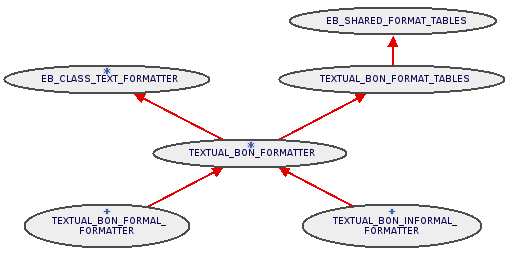
\includegraphics[scale=0.7]{images/textual-bon-formatter.png}
}
\caption{\textsc{textual$\textunderscore$bon$\textunderscore$formatter} inheritance relations.}
\label{fig:textual_bon_formatter}
\end{figure}

\begin{figure}[h]
\centerline{
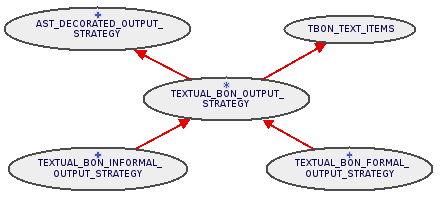
\includegraphics[scale=0.7]{images/bon-extraction-output-strategy.png}
}
\caption{\textsc{textual$\textunderscore$bon$\textunderscore$output$\textunderscore$strategy} inheritance relations.}
\label{fig:bon-extraction-output-strategy}
\end{figure}

\paragraph{}
The output strategies inherits a feature called \textit{process$\_$class$\_$as}. The purpose of this feature is to generate the desired output from a \textsc{class$\_$as}, which is the abstract eiffel syntax representation of a class. In the implementation of the \textsc{bon} tool, this is done by instantiating the previously mentioned meta-object (See figure \ref{fig:bon_extraction_3} on page \pageref{fig:bon_extraction_3}) from the \textsc{class$\_$as} object, which then generates the internal representation. This mechanism will be explained in detail in section \ref{tbon_class}.

\subsection{The Internal BON Representation}
\begin{figure}[h]
\centerline{
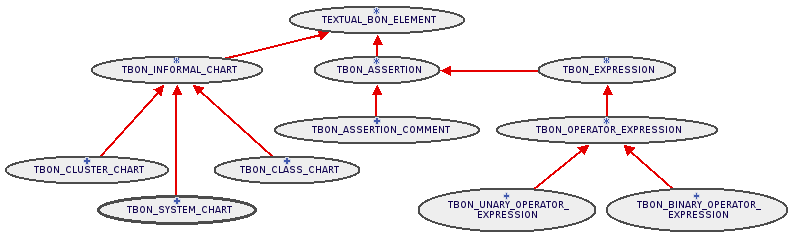
\includegraphics[scale=0.7]{images/bon-extractor-mog-overview.png}
}
\caption{An excerpt of the classes created for the internal representation of textual \bon{} in EiffelStudio. \textsc{tbon} is short for textual \bon.}
\label{fig:textual_bon_formatter}
\end{figure}
A series of classes has been created to represent the elements of the \bon{} grammar. Each of these classes store the information required about the represented grammar element in order to be able to generate textual \bon{}. The presence of mandatory elements of the grammar, such as a class name in a class chart, is ensured through the use of  \textit{attached} features and contracts (invariants and pre- and postconditions). A class thatrepresent a grammar element knows how to process itself, and itself only. If it contains other elements, such as a class containing features, the class will have a collection of features, and then delegate the processing of features to the class representing features. Any nested relations are processed this way.

\paragraph{}
This representation of textual \textsc{bon} is rooted in the \textsc{textual$\_$bon$\_$element} class. From this class, all classes inherit the features \textit{process$\_$to$\_$formal$\_$textual$\_$bon} and  \textit{process$\_$to$\_\newline$informal$\_$textual$\_$bon}. These features format textual \textsc{bon} based on the metadata in the enclosing class. For elements that only exist in either formal or informal \bon{} or have identical representations in the two, these two features have been renamed and joined into the same feature (\textit{process$\_$to$\_$textual$\_$bon}).

\subsubsection{Completeness}
To give a feeling of working with complete textual \bon{}, other parts than merely the class chart or the class component for the current class is generated. In the informal textual \bon{} view, both a system chart and cluster chart are created. A system chart keeps track of its contained cluster through a collection of clusters, and a cluster chart has a collection of clusters and classes. When a system chart is asked to process itself, it will also invoke the processing feature of its contained clusters, which then does the same for its contained classes and clusters. Analogous to the generation of a system chart and a cluster chart in the extraction of informal \bon{}, a cluster component is generated when extracting formal \bon{}.

\subsubsection{Indexing}
In order to translate the semantics of the indexing clause in Eiffel properly to informal textual \bon{}, a few alterations are made to it. Certain indexing tag names are identified as explanations and removed from the indexing clause and processed under the \textit{explanation} keyword of class charts in informal textual \bon{}. In the current implementation, the tags identified are \textit{description} and \textit{explanation} (the identificiation is not case-sensitive). This is identified by the feature \textit{is$\_$explanation$\_$string} in \textsc{tbon$\_$class$\_$chart}. Furthermore an extra entry into the indexing clause of a class chart is added to the informal textual \bon{}. To identify which cluster a class belongs to, a \textit{belongs$\_$to} tag has been added. This is not strictly necessary in this implementation, as one cluster is only ever made. However, if this was to be expanded to scale to a full system, one might want multiple clusters. As such, this tag provides the reader of the specification with a better overview.

\subsubsection{Inheritance}
To create an overview from the point of view of the currently selected class, specifications for all descendants of the current class is also extracted. This is done by inspecting the \textit{direct$\_$descendants} feature of the compiled class object from EiffelStudio (\textsc{class$\_$c}). These classes are then added to the cluster, and then processed into textual \bon{}.

\subsubsection{The Meta-Object}
\label{tbon_class}
When the output strategy receives the abstract Eiffel syntax, the internal \bon{} representation is created. As previously mentioned, this is done through a meta object. This object is denoted \textsc{tbon$\_$class}. \textsc{tbon$\_$class} takes a \textsc{class$\_$as} (abstract Eiffel representation of a class) object and instantiates the internal representation of the \bon{}. It does this by inspecting the abstract syntax represented by \textsc{class$\_$as} and parsing the information needed to the textual \bon{} objects.
\begin{figure}[H]
\centerline{
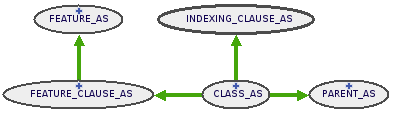
\includegraphics[scale=0.7]{images/abstract-syntax.png}
}
\caption{An example of the abstract Eiffel syntax.}
\label{fig:abstract-syntax}
\end{figure}

Figure \ref{fig:abstract-syntax} shows an example of a part of the abstract Eiffel syntax tree. In translation to the \bon{} internal representation (seen in figure \ref{fig:bon-rep}) one will notice a few differences or alterations. In the example is shown the representation of informal \bon. Since a class chart does not have the notion of feature clauses, but rather the idea of queries and commands, a class chart has a direct reference to a feature, rather than one going through a feature clause. The parent has been replaced by a reference to a class type which represents the notion of a class. Since all informal charts have indexing clauses, the class chart inherits this from the deferred informal chart class.
\begin{figure}[H]
\centerline{
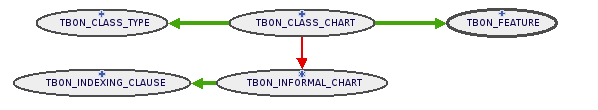
\includegraphics[scale=0.7]{images/bon-representation.png}
}
\caption{Example result of the meta-object extracting information from the abstract Eiffel syntax in figure \ref{fig:abstract-syntax}.}
\label{fig:bon-rep}
\end{figure}